\begingroup%
  \makeatletter%
  \providecommand\color[2][]{%
    \errmessage{(Inkscape) Color is used for the text in Inkscape, but the package 'color.sty' is not loaded}%
    \renewcommand\color[2][]{}%
  }%
  \providecommand\transparent[1]{%
    \errmessage{(Inkscape) Transparency is used (non-zero) for the text in Inkscape, but the package 'transparent.sty' is not loaded}%
    \renewcommand\transparent[1]{}%
  }%
  \providecommand\rotatebox[2]{#2}%
  \newcommand*\fsize{\dimexpr\f@size pt\relax}%
  \newcommand*\lineheight[1]{\fontsize{\fsize}{#1\fsize}\selectfont}%
  \ifx\svgwidth\undefined%
    \setlength{\unitlength}{329.25bp}%
    \ifx\svgscale\undefined%
      \relax%
    \else%
      \setlength{\unitlength}{\unitlength * \real{\svgscale}}%
    \fi%
  \else%
    \setlength{\unitlength}{\svgwidth}%
  \fi%
  \global\let\svgwidth\undefined%
  \global\let\svgscale\undefined%
  \makeatother%
  \begin{picture}(1,0.49658314)%
    \lineheight{1}%
    \setlength\tabcolsep{0pt}%
    \put(0,0){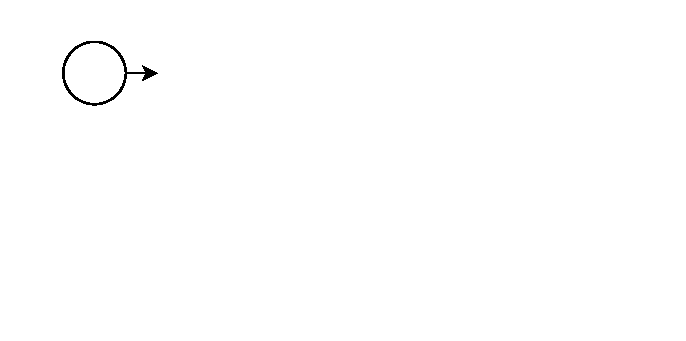
\includegraphics[width=\unitlength,page=1]{1-2.pdf}}%
    \put(0.13667426,0.38268793){\color[rgb]{0,0,0}\makebox(0,0)[t]{\lineheight{1.25}\smash{\begin{tabular}[t]{c}S\end{tabular}}}}%
    \put(0,0){\includegraphics[width=\unitlength,page=2]{1-2.pdf}}%
    \put(0.27334852,0.38268793){\color[rgb]{0,0,0}\makebox(0,0)[t]{\lineheight{1.25}\smash{\begin{tabular}[t]{c}A\end{tabular}}}}%
    \put(0,0){\includegraphics[width=\unitlength,page=3]{1-2.pdf}}%
    \put(0.27334852,0.23690205){\color[rgb]{0,0,0}\makebox(0,0)[t]{\lineheight{1.25}\smash{\begin{tabular}[t]{c}B\end{tabular}}}}%
    \put(0,0){\includegraphics[width=\unitlength,page=4]{1-2.pdf}}%
    \put(0.41002278,0.38268793){\color[rgb]{0,0,0}\makebox(0,0)[t]{\lineheight{1.25}\smash{\begin{tabular}[t]{c}$Q_{acc}$\end{tabular}}}}%
    \put(0,0){\includegraphics[width=\unitlength,page=5]{1-2.pdf}}%
    \put(0.18223235,0.30751708){\color[rgb]{0,0,0}\makebox(0,0)[t]{\lineheight{1.25}\smash{\begin{tabular}[t]{c}\small{0}\end{tabular}}}}%
    \put(0.38724374,0.30751708){\color[rgb]{0,0,0}\makebox(0,0)[t]{\lineheight{1.25}\smash{\begin{tabular}[t]{c}\small{01*0}\end{tabular}}}}%
    \put(0.27334852,0.45330296){\color[rgb]{0,0,0}\makebox(0,0)[t]{\lineheight{1.25}\smash{\begin{tabular}[t]{c}\small{1}\end{tabular}}}}%
    \put(0.27334852,0.17767654){\color[rgb]{0,0,0}\makebox(0,0)[t]{\lineheight{1.25}\smash{\begin{tabular}[t]{c}\small{1}\end{tabular}}}}%
    \put(0,0){\includegraphics[width=\unitlength,page=6]{1-2.pdf}}%
    \put(0.66059226,0.32346241){\color[rgb]{0,0,0}\makebox(0,0)[t]{\lineheight{1.25}\smash{\begin{tabular}[t]{c}S\end{tabular}}}}%
    \put(0,0){\includegraphics[width=\unitlength,page=7]{1-2.pdf}}%
    \put(0.79726651,0.32346241){\color[rgb]{0,0,0}\makebox(0,0)[t]{\lineheight{1.25}\smash{\begin{tabular}[t]{c}A\end{tabular}}}}%
    \put(0,0){\includegraphics[width=\unitlength,page=8]{1-2.pdf}}%
    \put(0.93394077,0.32346241){\color[rgb]{0,0,0}\makebox(0,0)[t]{\lineheight{1.25}\smash{\begin{tabular}[t]{c}$Q_{acc}$\end{tabular}}}}%
    \put(0,0){\includegraphics[width=\unitlength,page=9]{1-2.pdf}}%
    \put(0.79726651,0.39407745){\color[rgb]{0,0,0}\makebox(0,0)[t]{\lineheight{1.25}\smash{\begin{tabular}[t]{c}\small{1}\end{tabular}}}}%
    \put(0,0){\includegraphics[width=\unitlength,page=10]{1-2.pdf}}%
    \put(0.79726651,0.22551253){\color[rgb]{0,0,0}\makebox(0,0)[t]{\lineheight{1.25}\smash{\begin{tabular}[t]{c}\small{01*01*0}\end{tabular}}}}%
    \put(0,0){\includegraphics[width=\unitlength,page=11]{1-2.pdf}}%
    \put(0.27334852,0.03872437){\color[rgb]{0,0,0}\makebox(0,0)[t]{\lineheight{1.25}\smash{\begin{tabular}[t]{c}S\end{tabular}}}}%
    \put(0,0){\includegraphics[width=\unitlength,page=12]{1-2.pdf}}%
    \put(0.61503417,0.03872437){\color[rgb]{0,0,0}\makebox(0,0)[t]{\lineheight{1.25}\smash{\begin{tabular}[t]{c}$Q_{acc}$\end{tabular}}}}%
    \put(0.44419134,0.06378132){\color[rgb]{0,0,0}\makebox(0,0)[t]{\lineheight{1.25}\smash{\begin{tabular}[t]{c}\footnotesize{((1*)|(01*01*0)*)*}\end{tabular}}}}%
  \end{picture}%
\endgroup%
